\documentclass{beamer}

\usepackage{amsmath,amsthm,amsfonts}
\usepackage{mathrsfs,mathtools,mathdots}
\usepackage{caption,subcaption}
\usepackage{pgf,tikz}
%\usepackage{pgfplots}
%\usepackage{tikz-3dplot}
%\usetikzlibrary{shapes.geometric,arrows,arrows.meta,decorations.pathreplacing,bending}

\usetikzlibrary{positioning, decorations.markings}

\title{Algorithmic Graph Theory}
\author{Module III}
\institute{Chapter 5 : Networks}

\begin{document}

\begin{frame}
\maketitle
\end{frame}

\begin{frame}{Networks}
Network, $N$
\begin{enumerate}
	\item Digraph $D$ with two special vertices source and sink, $s \& t$.
	\item Capacity Function $c : E(D) \to \mathbb{Z}^+$.
\end{enumerate}

\begin{figure}[hbt]
\centering
\scalebox{0.8}{
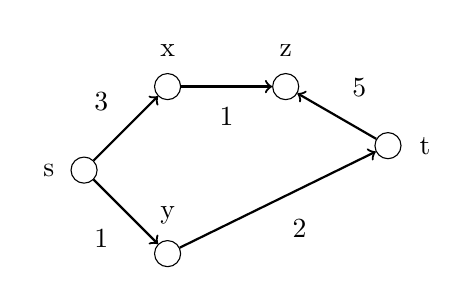
\begin{tikzpicture}
\begin{scope}
\tikzstyle every node=[draw,circle]
        \node (s)[label=left:s]{};
        \draw (s) ++(45:1.5) node (x)[label=x]{};
        \draw (s) ++(-45:1.5) node (y)[label=y]{};
        \draw (x) ++(0:1.5) node (z)[label=z]{};
        \draw (z) ++(-30:1.5) node (t)[label=right:t]{};
\end{scope}
        \draw[->,thick] (s)--node (e1)[sloped,label=above:3]{} (x);
        \draw[->,thick] (s)--node (e2)[sloped,label=below:1]{} (y);
        \draw[->,thick] (x)--node (e3)[sloped,label=below:1]{} (z);
        \draw[->,thick] (y)--node (e4)[sloped,label=below:2]{} (t);
        \draw[->,thick] (t)--node (e5)[sloped,label=5]{} (z);
\end{tikzpicture}
}
\end{figure}

Applications
\begin{enumerate}
	\item Logistics - Transportation Problem
	\item Flow Management - Oil Pipelines
\end{enumerate}
\end{frame}

\begin{frame}{Networks - Graph Theory}
\begin{description}
	\item[Out-neighbourhood] is the set of all out-neighbours.
	$$N^+(x) = \{ y \in V(D) : (x,y) \in E(D) \}$$
	\item[In-neighbourhood] is the set of all in-neighbours.
	$$N^-(x) = \{ y \in V(D) : (y,x) \in E(D) \}$$
	\item[Indegree] $id\ x = |N^-(x)|$.
	\item[Outdegree] $od\ x = |N^+(x)|$.
\end{description}
\end{frame}

\begin{frame}{Flow in a Network}
Flow is a function $f : E(D) \to \mathbb{Z}$ satisfying 
	\begin{enumerate}	
		\item Capacity Constraints
	$$ 0 \le f(a) \le c(a),\ \forall a \in E(D) $$
		\item Conservation of Flow
	$$ \sum_{y \in N^+(x)}\!\!\! f(x,y) = \sum_{y \in N^-(x)}\!\!\! f(y,x),\ \forall x \in V(D)-\{s,t\}$$ 
	\end{enumerate}
\end{frame}

\begin{frame}{Network with a Flow}
\begin{figure}[hbt]
\centering
\scalebox{0.8}{
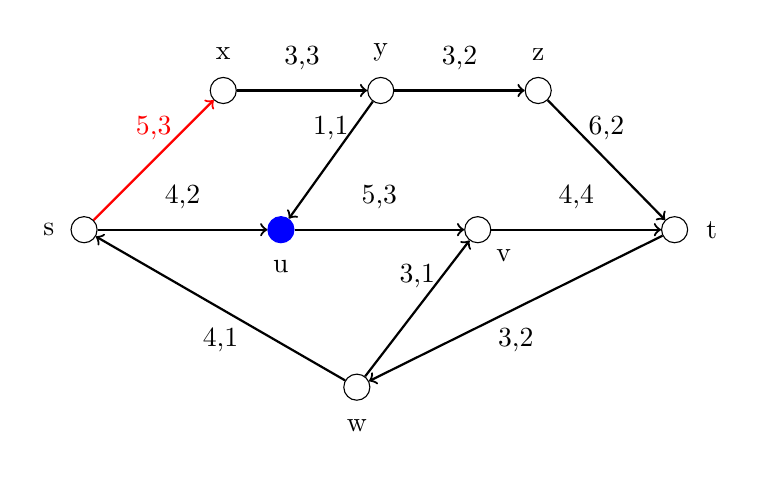
\begin{tikzpicture}
\tikzstyle arc=[draw,->,thick]
\begin{scope}
\tikzstyle every node=[draw,circle]
        \node (s)[label=left:s]{};
        \draw (s)++(45:2.5) node (x)[label=x]{};
	\draw (s)++(0:2.5) node[fill,blue] (u)[label=below:u]{};
        \draw (s)++(-30:4) node (w)[label=below:w]{};
        \draw (x)++(0:2) node (y)[label=y]{};
        \draw (y)++(0:2) node (z)[label=z]{};
        \draw (u)++(0:2.5) node (v)[label=below right:v]{};
        \draw (v)++(0:2.5) node (t)[label=right:t]{};
\end{scope}

        \path[arc,red] (s)--node (e1)[label=above:{5,3}]{} (x);
        \path[arc] (s)--node (e2)[label=above:{4,2}]{} (u);
        \path[arc] (w)--node (e3)[label=below:{4,1}]{} (s);
        \path[arc] (x)--node (e4)[label=above:{3,3}]{} (y);
        \path[arc] (y)--node (e5)[label=above:{1,1}]{} (u);
        \path[arc] (u)--node (e6)[label=above:{5,3}]{} (v);
        \path[arc] (w)--node (e7)[label=above:{3,1}]{} (v);
        \path[arc] (y)--node (e8)[label=above:{3,2}]{} (z);
        \path[arc] (z)--node (e9)[label=above:{6,2}]{} (t);
        \path[arc] (v)--node (ea)[label=above:{4,4}]{} (t);
        \path[arc] (t)--node (eb)[label=below:{3,2}]{} (w);
\end{tikzpicture}
}	
\end{figure}
\begin{itemize}
	\item {\color{red}$c(s,x) = 5$ and $f(s,x) = 3$.}
	\item {\color{blue}$f(s,u)+f(y,u) = f(u,v)$.}
\end{itemize}
\end{frame}

\begin{frame}{Flow and Cut}
	\begin{itemize}
		\item Flow in a Network, $f(N)$ is the flow out of source $s$.
		\item $f(N) = \only<1>{0} \only<2>{3} \only<3->{7}$ \only<4->{is the maximum flow}.
	\end{itemize}
\begin{figure}[hbt]
\centering
\scalebox{0.8}{
\begin{tikzpicture}
\tikzstyle arc=[draw,->,thick]
\begin{scope}
\tikzstyle every node=[draw,circle]
        \node (s)[label=left:s]{};
        \draw (s)++(45:2.5) node (x)[label=x]{};
	\draw (s)++(0:2.5) node (u)[label=below:u]{};
        \draw (s)++(-30:4) node (w)[label=below:w]{};
        \draw (x)++(0:2) node (y)[label=y]{};
        \draw (y)++(0:2) node (z)[label=z]{};
        \draw (u)++(0:2.5) node (v)[label=below right:v]{};
        \draw (v)++(0:2.5) node (t)[label=right:t]{};
\end{scope}

	\only<1,3->{\path[arc] (s)--node (e1)[label=above:{5,\only<1>{0}\only<2->{3}}]{} (x);}
	\only<2>{\path[arc,red] (s)--node (e1)[label=above:{5,3}]{} (x);}

	\only<1,2,4->{\path[arc] (s)--node (e2)[label=above:{4,\only<1,2>{0}\only<3->{4}}]{} (u);}
	\only<3>{\path[arc,red] (s)--node (e2)[label=above:{4,4}]{} (u);}

	\only<1->{\path[arc] (w)--node (e3)[label=below:{4,\only<1->{0}}]{} (s);}
	%\only<4>{\path[arc,red] (w)--node (e3)[label=below:{4,4}]{} (s);}

	\only<1,3->{\path[arc] (x)--node (e4)[label=above:{3,\only<1>{0}\only<2->{3}}]{} (y);}
	\only<2>{\path[arc,red] (x)--node (e4)[label=above:{3,3}]{} (y);}

	\only<1->{\path[arc] (y)--node (e5)[label=above:{1,\only<1->{0}}]{} (u);}
	%\only<4>{\path[arc,red] (y)--node (e5)[label=above:{1,4}]{} (u);}

	\only<1,2,4->{\path[arc] (u)--node (e6)[label=above:{5,\only<1,2>{0}\only<3->{4}}]{} (v);}
	\only<3>{\path[arc,red] (u)--node (e6)[label=above:{5,4}]{} (v);}

	\only<1->{\path[arc] (w)--node (e7)[label=above:{3,\only<1->{0}}]{} (v);}
	%\only<4>{\path[arc,red] (w)--node (e7)[label=above:{3,4}]{} (v);}

	\only<1,3->{\path[arc] (y)--node (e8)[label=above:{3,\only<1>{0}\only<2->{3}}]{} (z);}
	\only<2>{\path[arc,red] (y)--node (e8)[label=above:{3,3}]{} (z);}

	\only<1,3->{\path[arc] (z)--node (e9)[label=above:{6,\only<1>{0}\only<2->{3}}]{} (t);}
	\only<2>{\path[arc,red] (z)--node (e9)[label=above:{6,3}]{} (t);}

	\only<1,2,4->{\path[arc] (v)--node (ea)[label=above:{4,\only<1,2>{0}\only<3->{4}}]{} (t);}
	\only<3>{\path[arc,red] (v)--node (ea)[label=above:{4,4}]{} (t);}

	\only<1->{\path[arc] (t)--node (eb)[label=below:{3,\only<1->{0}}]{} (w);}
	%\only<4>{\path[arc,red] (t)--node (eb)[label=below:{3,4}]{} (w);}
\end{tikzpicture}
}	
\end{figure}
\end{frame}

\begin{frame}{Flow and Capacity between two Partitions}
\begin{itemize}
	\item Let $X,Y \subset V(D)$ such that $X \cap Y = \phi$ and $X \ne \phi$, $Y \ne \phi$.
	$$ f(X,Y) = \sum_{(x,y) \in (X,Y)} f(x,y) $$
	$$ c(X,Y) = \sum_{(x,y) \in (X,Y)} c(x,y) $$
\item {\color{red}For $X = \{s,y,w\}$, $f(X,Y) = 9$ and $c(X,Y) = 16$.}
\end{itemize}
\begin{figure}[hbt]
\centering
\scalebox{0.8}{
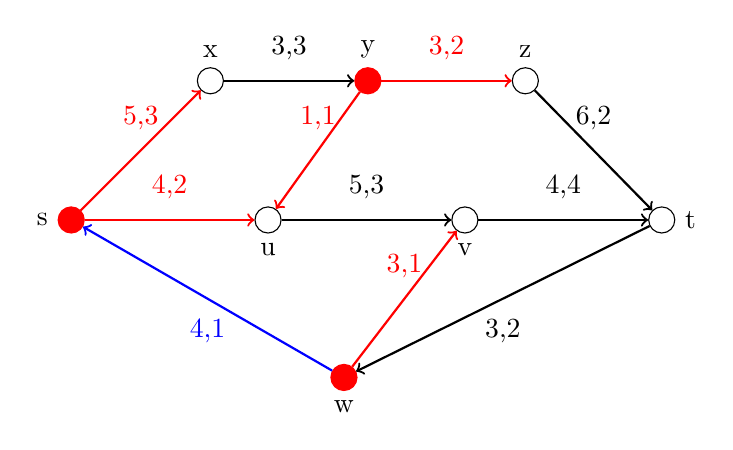
\begin{tikzpicture}
\tikzstyle show=[draw,circle]
\tikzstyle arc=[draw,->,thick]
	\node[fill,red] (s)[show,label=left:s]{};
	\draw (s)++(45:2.5) node (x)[show,label=x]{};
	\draw (s)++(0:2.5) node (u)[show,label=below:u]{};
	\draw (s)++(-30:4) node[fill,red] (w)[show,label=below:w]{};
	\draw (x)++(0:2) node[fill,red] (y)[show,label=y]{};
	\draw (y)++(0:2) node (z)[show,label=z]{};
	\draw (u)++(0:2.5) node (v)[show,label=below:v]{};
	\draw (v)++(0:2.5) node (t)[show,label=right:t]{};

	\path[arc,red] (s)--node (e1)[label=above:{5,3}]{} (x);
	\path[arc,red] (s)--node (e2)[label=above:{4,2}]{} (u);
	\path[arc,blue] (w)--node (e3)[label=below:{4,1}]{} (s);
	\path[arc] (x)--node (e4)[label=above:{3,3}]{} (y);
	\path[arc,red] (y)--node (e5)[label=above:{1,1}]{} (u);
	\path[arc] (u)--node (e6)[label=above:{5,3}]{} (v);
	\path[arc,red] (w)--node (e7)[label=above:{3,1}]{} (v);
	\path[arc,red] (y)--node (e8)[label=above:{3,2}]{} (z);
	\path[arc] (z)--node (e9)[label=above:{6,2}]{} (t);
	\path[arc] (v)--node (ea)[label=above:{4,4}]{} (t);
	\path[arc] (t)--node (eb)[label=below:{3,2}]{} (w);
\end{tikzpicture}
}
\end{figure}
\end{frame}

\begin{frame}{Theorem : Flow is restricted by the minimum cut}
	Cut $(P,\bar{P})$ is a partition of $V(D)$ such that $s \in P$ and $t \in \bar{P}$.

	\begin{theorem}
		Let $N$ be a network with flow $f(N)$ and $(P,\bar{P})$ be a cut in $N$. Then,
	$$f(N) = f(P,\bar{P}) - f(\bar{P},P)$$
	\end{theorem}

	\begin{corollary}
		Let $N$ be a network with flow $f(N)$. Then,
		$$f(N) \le \min c(P,\bar{P})$$
	\end{corollary}

	\begin{corollary}
		Let $N$ be a network with flow $f(N)$. Then,
		$$f(N)  = \sum_{x \in N^-(t)} f(x,t) - \sum_{x \in N^+(t)} f(t,x) $$
	\end{corollary}
\end{frame}

\begin{frame}{Max Flow Min Cut Theorem}
	\begin{itemize}
		\item A semipath is $f$-unsaturated if all forward arcs have more capacity than flow and all reverse arcs have positive flow.
		\item An $s-t$ semipath is $f$-augmenting if it is $f$-unsaturated.
	\end{itemize}

	\begin{theorem}[$f$-augmenting semipath]
		A flow in a network $f(N)$ is maximum if and only if there is no $f$-augmenting semipath in $D$.
	\end{theorem}

	\begin{theorem}[Max Flow Min Cut]
		Let $N$ be a network with maximum flow $f(N)$.
		Then $f(N)$ is equal to the capacity of the minimum cut $(P,\bar{P})$.
	\end{theorem}
\end{frame}

\begin{frame}{Proof : $f$-augmenting semipath}
	If there is an $f$-augmenting semipath $Q$ in $N$ then flow $f(N)$ can be further augmented. Thus, flow $f(N)$ is not maximum.
	\begin{itemize}
		\item Compute $\Delta$, maximum value that can be augmented along $Q$.
		\item $f^\ast$ with augmentation is a flow in network $N$.
		\begin{itemize}
			\item Case 0 : $x \notin Q$.
			\item Case 1 \& 2 : Both arcs enters/leaves $x$.
			\item Case 3 : One arc enters $x$ and Other leaves $x$
		\end{itemize}
	\end{itemize}
	\vfill	
	Suppose $f(N)$ has no $f$-augmenting path. And $f^\ast$ is maximum flow.
	\begin{itemize}
		\item $P = \left\{ x \in V(D) : \text{ there exists an $f$-augmenting path $s-x$ } \right\}$.
		\item $t \in \bar{P}$.
		\item $(P,\bar{P})$ is a cut in network $N$.
		\item $f(N) = f(P,\bar{P})-f(\bar{P},P) = f(P,\bar{P}) = c(P,\bar{P})$
		\item If $f^\ast$ is maximum flow and $(X,\bar{X})$ is minimum cut. Then $f(N) \le f^\ast(N) \le c(X,\bar{X}) \le C(P,\bar{P})$.
	\end{itemize}
\end{frame}

\begin{frame}
	\vspace{0.6in}
	\hspace{3cm} {\color{blue}\Huge{Thank You}}
\end{frame}
\end{document}

\begin{figure}[hbt]
\centering
\scalebox{0.8}{
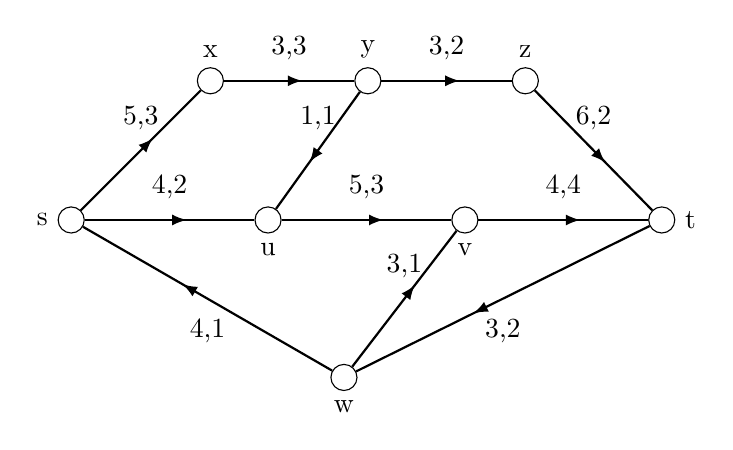
\begin{tikzpicture}
\tikzstyle show=[draw,circle]
\tikzset{arcs/.style={postaction={decorate}, decoration={markings,mark=at position #1  with {\arrow{latex}}, }}}
\tikzstyle arc=[draw,arcs=0.6,thick]
	\node (s)[show,label=left:s]{};
	\draw (s)++(45:2.5) node (x)[show,label=x]{};
	\draw (s)++(0:2.5) node (u)[show,label=below:u]{};
	\draw (s)++(-30:4) node (w)[show,label=below:w]{};
	\draw (x)++(0:2) node (y)[show,label=y]{};
	\draw (y)++(0:2) node (z)[show,label=z]{};
	\draw (u)++(0:2.5) node (v)[show,label=below:v]{};
	\draw (v)++(0:2.5) node (t)[show,label=right:t]{};

	\path[arc] (s)--node (e1)[label=above:{5,3}]{} (x);
	\path[arc] (s)--node (e2)[label=above:{4,2}]{} (u);
	\path[arc] (w)--node (e3)[label=below:{4,1}]{} (s);
	\path[arc] (x)--node (e4)[label=above:{3,3}]{} (y);
	\path[arc] (y)--node (e5)[label=above:{1,1}]{} (u);
	\path[arc] (u)--node (e6)[label=above:{5,3}]{} (v);
	\path[arc] (w)--node (e7)[label=above:{3,1}]{} (v);
	\path[arc] (y)--node (e8)[label=above:{3,2}]{} (z);
	\path[arc] (z)--node (e9)[label=above:{6,2}]{} (t);
	\path[arc] (v)--node (ea)[label=above:{4,4}]{} (t);
	\path[arc] (t)--node (eb)[label=below:{3,2}]{} (w);
\end{tikzpicture}
}
\caption{A network flow}
\label{dia:flow}
\end{figure}
